\chapter{Аналитический раздел}
В данном разделе будет рассмотрено описание работы алгоритмов нахождения межстрочного расстояния Левенштейна и Дамерау-Левенштейна.

\section{Описание алгоритмов}
Расстояние Левенштейна между двумя строками - это минимальное количество операций вставок (I), удалений (D) и замен (R) одного символа на другой, необходимых для преобразования одной строки в другую. Также в алгоритмах будет использоваться операция совпадения (M). Задачей алгоритмов, которые рассматриваются в этом разделе, является нахождение данного расстояния. В случае расстояния Дамерау-Левенштейна добавляется ещё одна операция - транспозиция (перестановка соседних символов, обозначается, как T).
\section{Расстояние Левенштейна}
Пускай у нас есть две строки $S_1$ и $S_2$, имеющие длину M и N соответственно. В таком случае расстояние Левенштейна может быть подсчитано по следующей рекуррентной формуле:

$D(S_1[1...i],S_2[1...j]) =$

\begin{equation}
	=\\
	\begin{cases}	
		0, &\text{$i = 0, j = 0$}\\
		$j$, &\text{$i = 0, j > 0$}\\
		$i$, &\text{$j = 0, i > 0$}\\
		min 
		\begin{cases}
			D(S_1[1...i],S_2[1...j-1]) + 1,\\
			D(S_1[1...i-1], S_2[1...j]) + 1, &\text{$j>0, i>0$}\\
			D(S_1[1...i-1], S_2[1...j-1]) + \\
			+
			\left[
		  		\begin{array}{ccc}
					$0, если $S_1$[i] = $S_2$[j]$\\
					$1, иначе R$
				\end{array}
			\right.
		\end{cases}
	\end{cases}
\end{equation}

При рассчёте разрешены следующие операции:
\begin{enumerate} 
	\item удаление (D, штраф - 1);
	\item удаление (I, штраф - 1);
	\item удаление (R, штраф - 1);
	\item удаление (M, штраф - 0).
\end{enumerate}

\section{Расстояние Дамерау-Левенштейна}
Алгоритм нахождения расстояния Дамерау-Левенштейна является модификацией расстояния Левенштейна. В частности ко множеству операций алгоритма расстояния Левенштейна была добавлена операция транспозиции (T) или перестановки символов. Данная модификация стала очевидно необходимой вследствие того, что значительная часть ошибок пользователей при наборе текста по сути является перестановкой символов.

Пускай у нас есть две строки $S_1$ и $S_2$, имеющие длину M и N соответственно. В таком случае расстояние Дамерау-Левенштейна может быть подсчитано по следующей рекуррентной формуле:

$D(S_1[1...i],S_2[1...j]) =$

\begin{equation}
	=\\
	\begin{cases}	
		0, &\text{$i = 0, j = 0$}\\
		$j$, &\text{$i = 0, j > 0$}\\
		$i$, &\text{$j = 0, i > 0$}\\
		min 
		\begin{cases}
			D(S_1[1...i],S_2[1...j-1]) + 1,\\
			D(S_1[1...i-1], S_2[1...j]) + 1, &\text{$j>0, i>0$}\\
			D(S_1[1...i-1], S_2[1...j-1]) + \\
			+
			\left[
		  		\begin{array}{ccc}
					$0, если $S_1$[i] = $S_2$[j]$\\
					$1, иначе R$
				\end{array}
			\right.\\
			D(S_1[1...i-2], S_2[1...j-2]) + 1, $  если$ j>1, i>1\\ $ и $ S_1[i] = S_2[j - 1], S_1[i - 1] = S_2[j]\\
		\end{cases}
	\end{cases}
\end{equation}

\section{Вывод}
В данном разделе выбли рассмотрены расстояния Левенштейна и Дамерау-Левенштейна. Были приведены формулы, позволяющие вычислить оба расстояния. Была указана разница между расстоянием Левенштейна и расстоянием Дамерау-Левенштейна, заключающаяся в добавлении операции транспозиции, а также причины, приведшие к появлению этой разницы. В результате добавления этой операции области применения расстояния Левенштейна и расстояния Дамерау-Левенштейна могут различаться. В качестве входных данных оба алгоритма получают на вход две строки, причём длина обеих строк может быть как равна нулю, так и достигать максимально допустимой для реализации алгоритма. На выходе данные алгоритмы возвращают целое число - минимальное редакторское расстояние между строками.

\chapter{Конструкторский раздел}

В данном разделе будут рассмотрены схемы, структуры данных, способы тестирования, описания памяти для следующих алгоритмов:
\begin{enumerate}
	\item нерекурсивный алгоритм поиска расстояния Левенштейна (табличный
способ);
	\item рекурсивный алгоритм поиска расстояния Левенштейна без заполнения
матрицы;
	\item рекурсивный алгоритм поиска расстояния Левенштейна с заполнением
и дополнительными проверками матрицы;
	\item нерекурсивный алгоритм поиска расстояния Дамерау-Левенштейна
(табличный способ).
\end{enumerate}

Общие замечания для всех алгоритмов:
\begin{enumerate}
	\item сложные структуры данных не будут использоваться, так как в них нету необходимости;
	\item все описанные выше алгоритмы в качестве результата возращают число - посчитаное минимальное редакторское расстояние;
\end{enumerate}

\section{Тестирование алгоритмов}
Выделение классов эквивалентности для тестирования алгоритмов:
\begin{enumerate}
	\item проверка на пустых строках;
	\item проверка на одну пустую строку;
	\item проверка на одинаковых строках;
	\item проверка на общем случае.
\end{enumerate}

Описание тестов:
\begin{enumerate}
	\item обе строки, подающиеся на вход, пустые;
	\item певая строка, подающаяся на вход, пустая;
	\item вторая строка, подающаяся на вход, пустая;
	\item на вход подаются две разные непустые строки;
	\item на вход подаются две одинаковые непустые строки.
\end{enumerate}

\section{Нерекурсивный алгоритм поиска расстояния Левенштейна (табличный
способ)}

Описание типов и структур данных, используемых в алгоритме:
\begin{enumerate}
	\item строковые переменные, представляющая из себя массив символов;
	\item целочисленные переменные, использующаяся для хранения индексов и результата
	\item массивы целых числел, использующиеся как кэш-строки
\end{enumerate}

Алгоритм поиска расстояния Левенштейна подразумевает использование таблицы для вычисления редакторского расстояния. Однако для экономии памяти будут использоваться только два кэш-массива. Данные массивы будут иметь длину равную длине первой строки, и будут содержать целочисленные значения. Также помимо этих массивов в программе будут использоваться две строки a и b, подающиеся на вход функции, локальные целочисленные переменные n, m, хранящие длину поданных на вход строк и локальные целочисленные переменные I, D, R - хранящие промежуточные результаты операций при итерации вычисления редакторского расстояния.

\begin{figure}[ph!]
	\center{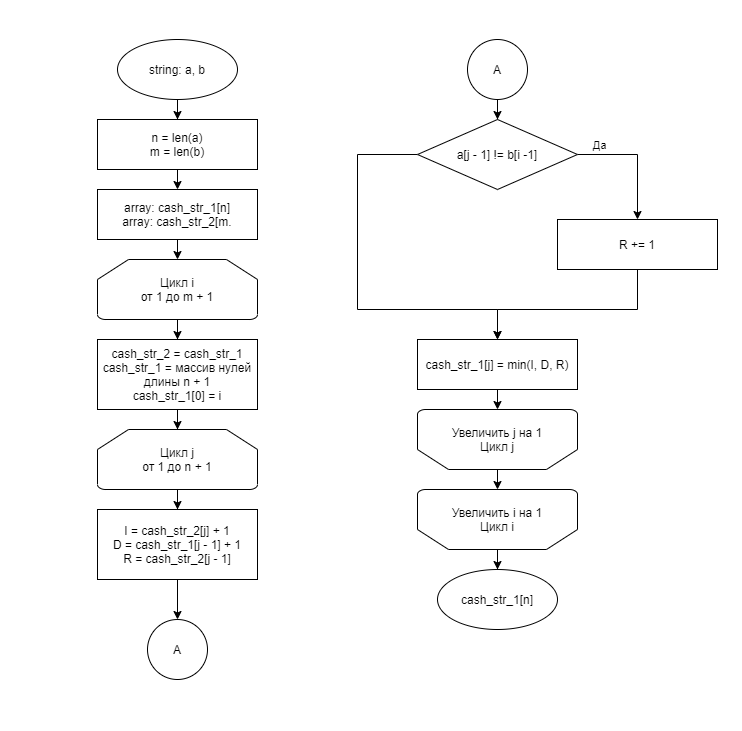
\includegraphics[scale=0.4]{lev_table}}
	\caption{Схема нерекурсивного алгоритма поиска расстояния Левенштейна табличным способом.}
\end{figure}

\newpage

\section{Рекурсивный алгоритм поиска расстояния Левенштейна без заполнения
матрицы}

Описание типов и структур данных, используемых в алгоритме:
\begin{enumerate}
	\item строковые переменные, представляющая из себя массив символов;
	\item целочисленные переменные, использующаяся для хранения индексов и результата
\end{enumerate}

Рекурсивный алгоритм Левенштейна использует одну локальную целочисленную переменную - result, хранящую результат выполнения очередной итерации вычисления редакторского расстояния. Также используются две строковые переменные a и b, хранящие поданные на вход функции строки.

\begin{figure}[ph!]
	\center{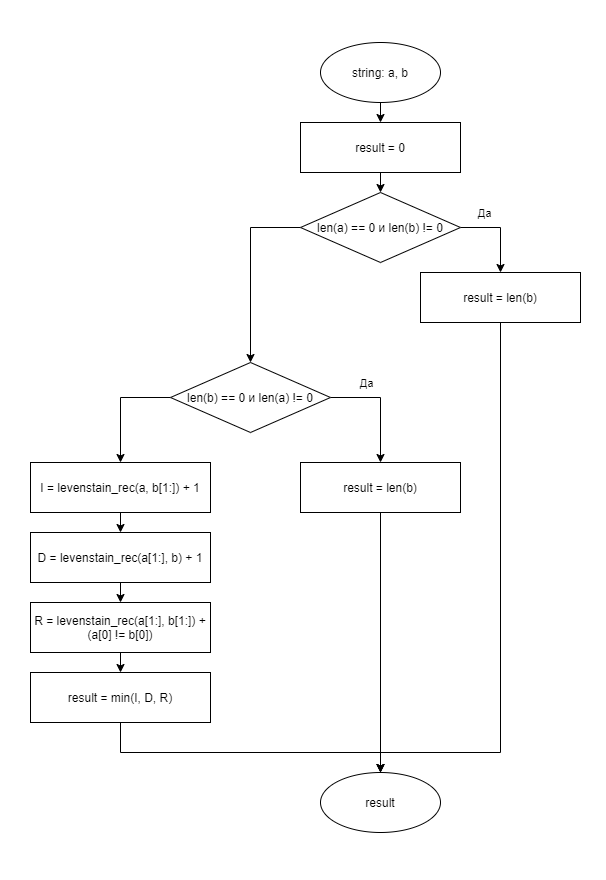
\includegraphics[scale=0.4]{lev_rec}}
	\caption{Схема рекурсивного алгоритма поиска расстояния Левенштейна без заполнения матрицы.}
\end{figure}
\newpage

\section{Рекурсивный алгоритм поиска расстояния Левенштейна с заполнением и дополнительными проверками матрицы}

Описание типов и структур данных, используемых в алгоритме:
\begin{enumerate}
	\item строковые переменные, представляющая из себя массив символов;
	\item целочисленные переменные, использующаяся для хранения индексов и результата
	\item массив массивов целых чисел, использующийся как таблица при вычислении результата
\end{enumerate}

Для работы данного алгоритма при каждом рекурсивном вызове функции необходимо помимо строк передавать индексы i, j и само тело матрицы. Мы не будем делать проверку внутри функции, поскольку это приведёт к излишним временным затратам, к тому же мы можем быть уверены, что после первой итерации алгоритма в функцию будут передаваться верные значения. В качестве входных параметров фукцния получает две строковые переменные a, b, два целочисленных числа - i, j, и целочисленную матрицу mat, имеющую размер [len(b) + 1, len(a) + 1]. Также внутри функции есть локальные целочисленные переменные result и R. result хранит результат работы функции. R - хранит число, добавляемое при вычислении стоимости операции.
\newpage
\begin{figure}[ph!]
	\center{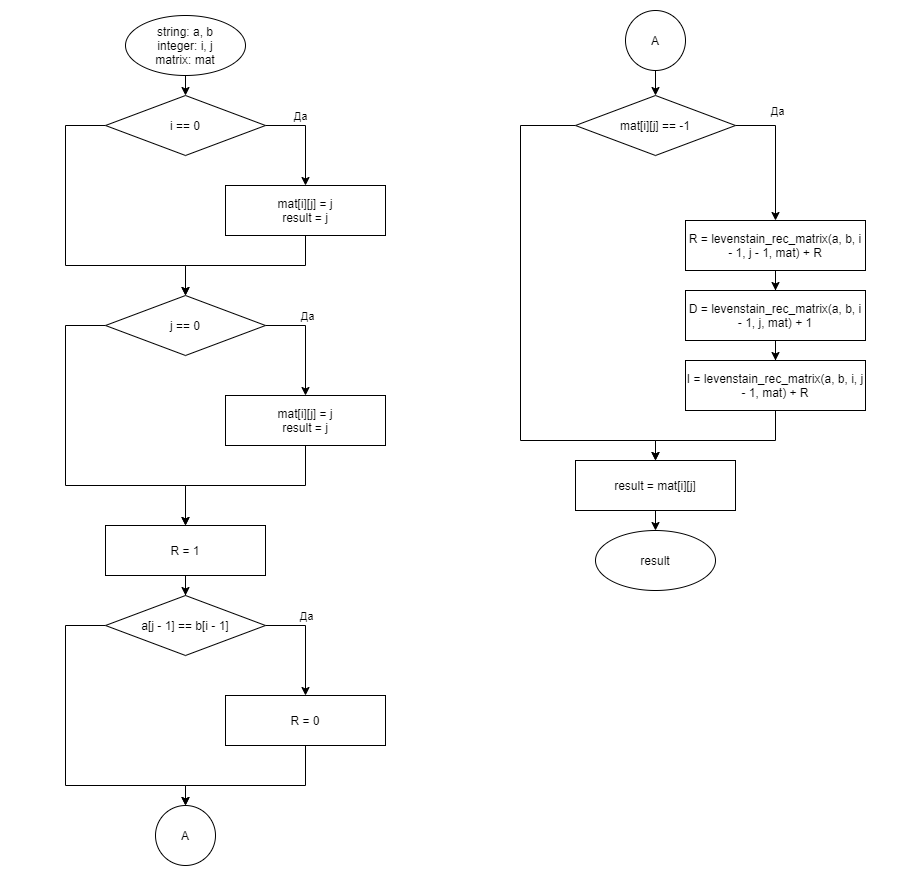
\includegraphics[scale=0.5]{lev_rec_matrix}}
	\caption{Схема рекурсивного алгоритма поиска расстояния Левенштейна с заполнением и дополнительными проверками матрицы.}
\end{figure}
\newpage
\section{Нерекурсивный алгоритм поиска расстояния Дамерау-Левенштейна (табличный способ)}

Описание типов и структур данных, используемых в алгоритме:
\begin{enumerate}
	\item строковые переменные, представляющая из себя массив символов;
	\item целочисленные переменные, использующаяся для хранения индексов и результата
	\item массив массивов целых чисел, использующийся как таблица при вычислении результата
\end{enumerate}

Алгоритм поиска расстояния Дамерау-Левенштейна подразумевает использование таблицы для вычисления редакторского расстояния. В данном случае будет использоваться таблица целых чисел mat, имеющая размер n на m, где n и m - локальные целочисленные переменные, равные длине подаваемых на вход функции строк a и b соответственно. Помимо этого в программе используется локальная целочисленная переменная R, использующаяся для хранения значения, использующегося при вычислении стоимости операций замены и транспозиции.

\begin{figure}[ph!]
	\center{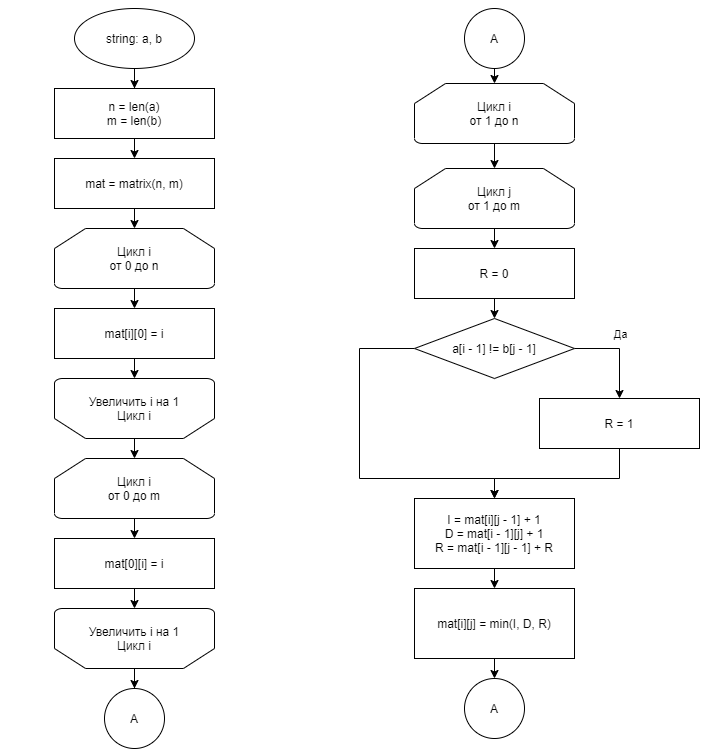
\includegraphics[scale=0.35]{damerau_lev_table}}
	\caption{Схема нерекурсивного алгоритма поиска расстояния Дамерау-Левенштейна табличным способом. Часть 1.}
\end{figure}
\newpage
\begin{figure}[ph!]
	\center{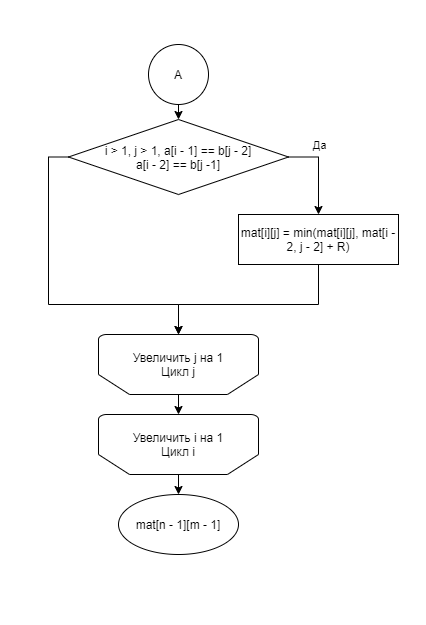
\includegraphics[scale=0.5]{damerau_lev_table_p2}}
	\caption{Схема нерекурсивного алгоритма поиска расстояния Дамерау-Левенштейна табличным способом. Часть 2.}
\end{figure}
\newpage
\section{Функциональная схема ПО}
\begin{figure}[ph!]
	\center{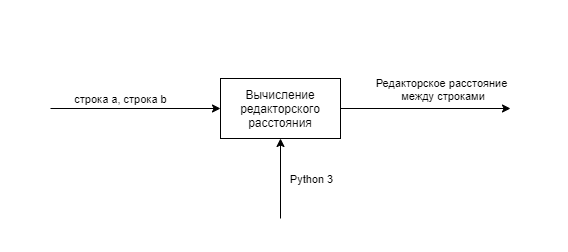
\includegraphics[scale=1.0]{idef_0}}
	\caption{Схема нерекурсивного алгоритма поиска расстояния Дамерау-Левенштейна табличным способом. Часть 2.}
\end{figure}


\section{Вывод}
В данном разделе были рассмотрены схемы алгоритмов для каждого из способов вычисления редакторского расстояния, и были определены общие тесты для каждого алгоритма, юыли описаны типы и вид входных данных. Помимо этого были выделены и описаны особенности реализации алгоритмов, в которых используются дополнительные структуры данных для хранения и обработки информации при вычислении редакторского расстояния (кэш-строки в табличном способе вычисления расстояния Левенштейна, матрица в рекурсивном способе вычисления алгоритма Левенштейне, таблица табличном способе вычисления алгоритма Дамерау-Левенштейне).

\chapter{Технологический раздел}

В данном разделе будут рассмотрены подробности реализации описаных выше алгоритмов. Также будут обоснованы выбор языка программирования для реализации, выбор библиотек для проведения экспериментов и представлены важные фрагменты кода написанной в рамках работы программы.

\section{Выбор языка программирования}

В качестве языка программирования для реализации данной лабораторной работы использовался язык программирования python (3.9.7) [1] в целях упрощения работы со структурами данных и визцализацией данных сравнительных анализов и наличием опыта работы с данным языком программирования. В качестве среды разработки использовалась Visual Studio Code [2]. Для замеров процедурного времени использовалась функция process\_time() из библиотеки time [3].

\section{Сведения о модулях программы}

Реализованное ПО состоит из трёх модулей:
\begin{enumerate}
	\item algos.py - в данном модуле реализованы алгоритмы рассчёта редакторского расстояния;
	\item time.py- в данном модуле реализованы замеры временных характеристик алгоритмов;
	\item test.py - в данном модуле реализованы тесты программ.
\end{enumerate}

\section{Реализация алгоритмов поиска редакторского расстояния}

\begin{lstlisting}[label=some-code-1,caption=Реализация нерекурсивного алгоритма поиска расстояния Левенштейна табличным способом.]
def levenstain_table(a, b):
    n, m = len(a), len(b)
    cash_str_1 = [*range(n + 1)]
    cash_str_2 = [*range(n + 1)]

    for i in range(1, m + 1):
        cash_str_2 = cash_str_1
        cash_str_1 = [i] + [0] * n
        for j in range(1, n + 1):
            I = cash_str_2[j] + 1
            D = cash_str_1[j - 1] + 1
            R = cash_str_2[j - 1]
            if a[j - 1] != b[i - 1]:
                R += 1
            cash_str_1[j] = min(I, D, R)
    return cash_str_1[n]
\end{lstlisting}

\begin{lstlisting}[label=some-code-2,caption=Реализация рекурсивного алгоритма поиска расстояния Левенштейна без заполнения матрицы.]
def levenstain_rec(a, b):
    result = 0
    if len(a) == 0 and len(b) == 0:
        result = 0
    elif len(a) == 0 and len(b) != 0:
        result = len(b)
    elif len(b) == 0 and len(a) != 0:
        result = len(a)
    else:
        result = min(
            levenstain_rec(a, b[1:]) + 1,
            levenstain_rec(a[1:], b) + 1,
            levenstain_rec(a[1:], b[1:]) + (a[0] != b[0])
        )
    return result

\end{lstlisting}

\begin{lstlisting}[label=some-code-3,caption=Реализация  рекурсивного алгоритма поиска расстояния Левенштейна с заполнением и дополнительными проверками матрицы.]
def levenstain_rec_matrix(a, b, i, j, mat):
    result = 0
    if len(a) == 0 and len(b) == 0:
        result = 0
    elif i == 0:
        mat[i][j] = j
        result = j
    elif j == 0:
        mat[i][j] = i
        result = i
    else:
        R = 1
        if a[j - 1] == b[i - 1]:
            R = 0

        if mat[i][j] == -1:
            mat[i][j] = min(
                levenstain_rec_matrix(a, b, i - 1, j - 1, mat) + R, # R
                levenstain_rec_matrix(a, b, i - 1, j, mat) + 1, # D
                levenstain_rec_matrix(a, b, i, j - 1, mat) + 1 # I
                )
        result = int(mat[i][j])
    return result
\end{lstlisting}

\begin{lstlisting}[label=some-code-4,caption=Реализация нерекурсивного алгоритма поиска расстояния Дамерау-Левенштейна табличным способом.]
def damerau_levenstain_table(a, b):
    n = len(a) + 1
    m = len(b) + 1
    mat = np.zeros([n, m]).astype(int)
    
    for i in range(0, n):
        mat[i, 0] = i
    for i in range(0, m):
        mat[0, i] = i

    for i in range(1, n):
        for j in range(1, m):
            R = 0
            if a[i - 1] != b[j - 1]:
                R = 1
            mat[i][j] = min(
                mat[i][j - 1] + 1, # I
                mat[i - 1][j] + 1, # D
                mat[i - 1][j - 1] + R # R
            )
            if (i > 1 and j > 1) and a[i - 1] == b[j - 2] and a[i - 2] == b[j - 1]:
                mat[i][j] = min(mat[i][j], mat[i - 2][j - 2] + R) # T
    return mat[n - 1][m - 1]
\end{lstlisting}

\section{Реализация тестирования алгоритмов}

Для тестирования алгоритмов было реализовано несколько тесто для каждого класса эквивалентности:
\begin{enumerate}
	\item обе строки, подающиеся на вход, пустые;
	\item первая из строк, подающихся на вход, пустая, вторая имеет ненулевую длину;
	\item вторая из строк, подающихся на вход, пустая, первая имеет ненулевую длину;
	\item обе строки, подающиеся на вход, имеют одинаковую ненулевую длину;
	\item обе строки, подающиеся на вход, имеют разную ненулевую длину.
\end{enumerate}

\begin{lstlisting}[label=some-code-5,caption=Реализация функции рандомной генерации строк.]
def str_gen(str_len):
    src_str = string.ascii_lowercase
    return ''.join(random.choice(src_str) for i in range(str_len))

\end{lstlisting}

\begin{lstlisting}[label=some-code-6,caption=Реализация тестирования на пустых строках.]
def test_empty():
    a = ''
    b = ''
    mat_lrm = np.zeros([len(b) + 1, len(a) + 1]).astype(int)
    mat_lrm.fill(-1)
    return levenstain_table(a, b) == 0 and levenstain_rec(a, b) == 0\
         and levenstain_rec_matrix(a, b, len(b), len(a), mat_lrm) == 0 and\
              damerau_levenstain_table(a, b) == 0
\end{lstlisting}

\begin{lstlisting}[label=some-code-7,caption=Реализация тестирования первой пустой строки.]
def test_first(test_len):
    a = ''
    b = str_gen(test_len)
    mat_lrm = np.zeros([len(b) + 1, len(a) + 1]).astype(int)
    mat_lrm.fill(-1)
    return levenstain_table(a, b) == len(b) and levenstain_rec(a, b) == len(b)\
         and levenstain_rec_matrix(a, b, len(b), len(a), mat_lrm) == len(b) and\
              damerau_levenstain_table(a, b) == len(b)
\end{lstlisting}

\begin{lstlisting}[label=some-code-8,caption=Реализация тестирования второй пустой строки.]
def test_second(test_len):
    a = str_gen(test_len)
    b = ''
    mat_lrm = np.zeros([len(b) + 1, len(a) + 1]).astype(int)
    mat_lrm.fill(-1)
    return levenstain_table(a, b) == len(a) and levenstain_rec(a, b) == len(a)\
         and levenstain_rec_matrix(a, b, len(b), len(a), mat_lrm) == len(a) and\
              damerau_levenstain_table(a, b) == len(a)
\end{lstlisting}

\begin{lstlisting}[label=some-code-9,caption=Реализация тестирования строк равной ненулевой длины.]
def test_equal(test_len):
    a = str_gen(test_len)
    b = a
    mat_lrm = np.zeros([len(b) + 1, len(a) + 1]).astype(int)
    mat_lrm.fill(-1)
    return levenstain_table(a, b) == 0 and levenstain_rec(a, b) == 0\
         and levenstain_rec_matrix(a, b, len(b), len(a), mat_lrm) == 0 and\
              damerau_levenstain_table(a, b) == 0
\end{lstlisting}

\begin{lstlisting}[label=some-code-10,caption=Реализация тестирования строк разной ненулевой длины.]
def test_diff(test_len, diff_len):
    a = str_gen(test_len)
    b = str_gen(test_len + diff_len)
    mat_lrm = np.zeros([len(b) + 1, len(a) + 1]).astype(int)
    mat_lrm.fill(-1)
    return levenstain_table(a, b) == levenstain_rec(a, b) == \
        levenstain_rec_matrix(a, b, len(b), len(a), mat_lrm) == damerau_levenstain_table(a, b)
\end{lstlisting}

\section{Сравнительный анализ потребляемой памяти}
Для того, чтобы провести анализ, нам необходимо знать количество потребляемой памяти для различных классов величин.

\begin{table}[h!]
  \begin{center}
    \caption{Количество потребляемой памяти для различных классов величин.}
    \label{tab:table1}
    \begin{tabular}{c|c|c}
      \textbf{Классы элементов} & \textbf{Представление в коде} & \textbf{Занимаемая память в байтах}\\
      \hline
	Пустой numpy массив & [] & 48\\
	Numpy массив длины 5, заполненный нулями & [0, 0, 0, 0, 0] & 88\\
	Numpy массив с массивом & [[]] & 56\\
	Целое число & Int(10) & 14\\
	Пустая строка & Str("") & 25
    \end{tabular}
  \end{center}
\end{table}

Как мы можем увидеть, хранение элементов массива реализовано с помощью указателей, в связи с чем для вложенных массивов требуется отдельный подсчёт занимаемой памяти.

Посчитаем минимальный объём потребляемой памяти для каждого алгоритма:

Алгоритм Левенштейна нерекурсивный табличный:
\begin{itemize}
	\item два кэш-массива - 48 * 2 + 8 * (len(str\_1) + 1) + 8 * (len(str\_2 + 1)) байт;
	\item пять вспомогательных целочисленных переменных - 70 байт;
	\item два целочисленных счётчика - 28 байт;
	\item передача двух строк - 50 байт.
\end{itemize}

Алгоритм Левенштейна рекурсивный:
\begin{itemize}
	\item целочисленная переменная для хранения результата - 14 байт;
	\item передача двух строк - 50 байт.
\end{itemize}

Алгоритм Левенштейна рекурсивный с проверками матрицы:
\begin{itemize}
	\item передача входных параметров - 25 + 25 + 14 * 2 + 48 = 122 байта;
	\item две вспомогательные целочисленные переменные - 14 * 2 = 28 байт;
	\item целочисленная матрица - 48 + 8 * (len(str\_2) + 1) * (len(str\_1) + 1).
\end{itemize}

Алгоритм Дамерау-Левенштейна:
\begin{itemize}
	\item передача входных параметров - 25 + 25 = 50 байт;
	\item вспомогательные целочисленные переменные - 14 * 3 = 42 байта;
	\item два целочисленных счётчика - 14 * 2 = 28 байт;
	\item целочисленная матрица - 48 + 8 * (len(str\_2) + 1) * (len(str\_1) + 1).
\end{itemize}

Оценим потребляемую память на словах длиной в 5 и 100 символов.
Для слов, длиной в 5 символов:

Алгоритм Левенштейна нерекурсивный табличный:
\begin{itemize}
	\item два кэш-массива - 48 * 2 + 8 * 6 + 8 * 6 = 182 байта;
	\item пять вспомогательных целочисленных переменных - 70 байт;
	\item два целочисленных счётчика - 28 байт;
	\item передача двух строк - 50 байт.
\end{itemize}

Алгоритм Левенштейна рекурсивный:
\begin{itemize}
	\item целочисленная переменная для хранения результата - 14 * 10 байт;
	\item передача двух строк - 50 * 10 байт.
\end{itemize}

Алгоритм Левенштейна рекурсивный с проверками матрицы:
\begin{itemize}
	\item передача входных параметров - 25 + 25 + 14 * 2 + 48 = 122 * 25 = 3050 байта;
	\item две вспомогательные целочисленные переменные - 14 * 2 = 28 * 25 = 700 байт;
	\item целочисленная матрица - 48 + 8 * 6 * 6 = 336 байт.
\end{itemize}

Алгоритм Дамерау-Левенштейна:
\begin{itemize}
	\item передача входных параметров - 25 + 25 = 50 байт;
	\item вспомогательные целочисленные переменные - 14 * 3 = 42 байта;
	\item два целочисленных счётчика - 14 * 2 = 28 байт;
	\item целочисленная матрица - 48 + 8 * 6 * 6 = 336 байт.
\end{itemize}

Для слов, длиной в 500 символов:

Алгоритм Левенштейна нерекурсивный табличный:
\begin{itemize}
	\item два кэш-массива - 48 * 2 + 8 * 501 + 8 * 501 = 4104 байт;
	\item пять вспомогательных целочисленных переменных - 70 байт;
	\item два целочисленных счётчика - 28 байт;
	\item передача двух строк - 50 байт.
\end{itemize}

Алгоритм Левенштейна рекурсивный:
\begin{itemize}
	\item целочисленная переменная для хранения результата - 14 * 500 байт;
	\item передача двух строк - 50 * 500 байт.
\end{itemize}

Алгоритм Левенштейна рекурсивный с проверками матрицы:
\begin{itemize}
	\item передача входных параметров - 25 + 25 + 14 * 2 + 48 = 122 байта;
	\item две вспомогательные целочисленные переменные - 14 * 2 = 28 байт;
	\item целочисленная матрица - 48 + 8 * 501 * 501 = 2008056 байт.
\end{itemize}

Алгоритм Дамерау-Левенштейна:
\begin{itemize}
	\item передача входных параметров - 25 + 25 = 50 байт;
	\item вспомогательные целочисленные переменные - 14 * 3 = 42 байта;
	\item два целочисленных счётчика - 14 * 2 = 28 байт;
	\item целочисленная матрица - 48 + 8 * 501 * 501.
\end{itemize}

\begin{table}[h!]
  \begin{center}
 \captionsetup{justification=raggedright}
    \caption{Результаты сравнения количества потребляемой памяти для 5 символов.}
    \label{tab:table2}
    \begin{tabular}{c|c}
      \textbf{Алгоритм} & \textbf{Занимаемая память в байтах}\\
      \hline
	Левенштейна нерекурсивный табличный & 330\\
	Левенштейна рекурсивный & 640\\
	Левенштейна рекурсивный с проверками матрицы & 4086\\
	Дамерау-Левенштейна & 456\\
    \end{tabular}
  \end{center}
\end{table}


\begin{table}[h!]
  \begin{center}
 \captionsetup{justification=raggedright}
    \caption{Результаты сравнения количества потребляемой памяти для 500 символов.}
    \label{tab:table3}
    \begin{tabular}{c|c}
      \textbf{Алгоритм} & \textbf{Занимаемая память в байтах}\\
      \hline
	Левенштейна нерекурсивный табличный & 4252\\
	Левенштейна рекурсивный & 32000\\
	Левенштейна рекурсивный с проверками матрицы & 2008206\\
	Дамерау-Левенштейна & 2008176\\
    \end{tabular}
  \end{center}
\end{table}

\section{Вывод}
В данном разделе была представлена реализация алгоритмов нахождения расстояния Левенштейна (нерекурсивный способ, рекурсивный способ, рекурсивный способ с заполнением и дополнительные проверками матрицы), а также Дамерау-Левенштейна (табличный способ). Были разработаны алгоритмы тестирования разработанных методов по методу чёрного ящика. Был проведён анализ потребляемой памяти, в ходе которого был сделан вывод о том, что классический алгоритм, реализованный с использованием двух кэш-массивов, эффективнее по памяти, чем остальные алгоритмы.

\chapter{Экспериментальный раздел}

В данном разделе будет изучено влияние длины подаваемых на вход строк на время выполнения программы. Также будет проведено сравнение полученных результатов и сделаны выводы о временной эффективности данных алгоритмов.

\section{Измерение временных характеристик для рекурсивного алгоритма Левенштейна с проверками и заполнением матрицы, нерекурсивного Левенштейна, Дамерау-Левенштейна}

Для измерения времени данных алгоритмов будет использовать рандомно генерирующиеся строки длиной от 100 до 500 с шагом 100. Для более точных измерений, для каждой длины замеры будут проводиться 50 раз и в результат будет заноситься средняя величина.

\begin{table}[h!]
  \begin{center}
 \captionsetup{justification=raggedright}
    \caption{Результаты временных тестов.}
    \label{tab:table4}
    \begin{tabular}{c|c|c|c}
	\textbf{Длина строки} & \textbf{Левенштейн нерекурсивный табличный} & \textbf{Левенштейн рекурсивный с проверками матриц} & \textbf{Дамерау-Левенштейна}\\
      \hline
	100 & 0.0040625 & 0.03375 & 0.01625\\
	200 & 0.01625 & 0.114375 & 0.064375\\
	300 & 0.0353125 & 0.2653125 & 0.14875\\
	400 & 0.06875 & 0.4675 & 0.271875\\
	500 & 0.115625 & 0.7459375 & 0.45\\
    \end{tabular}
  \end{center}
\end{table}

\begin{figure}[ph!]
	\center{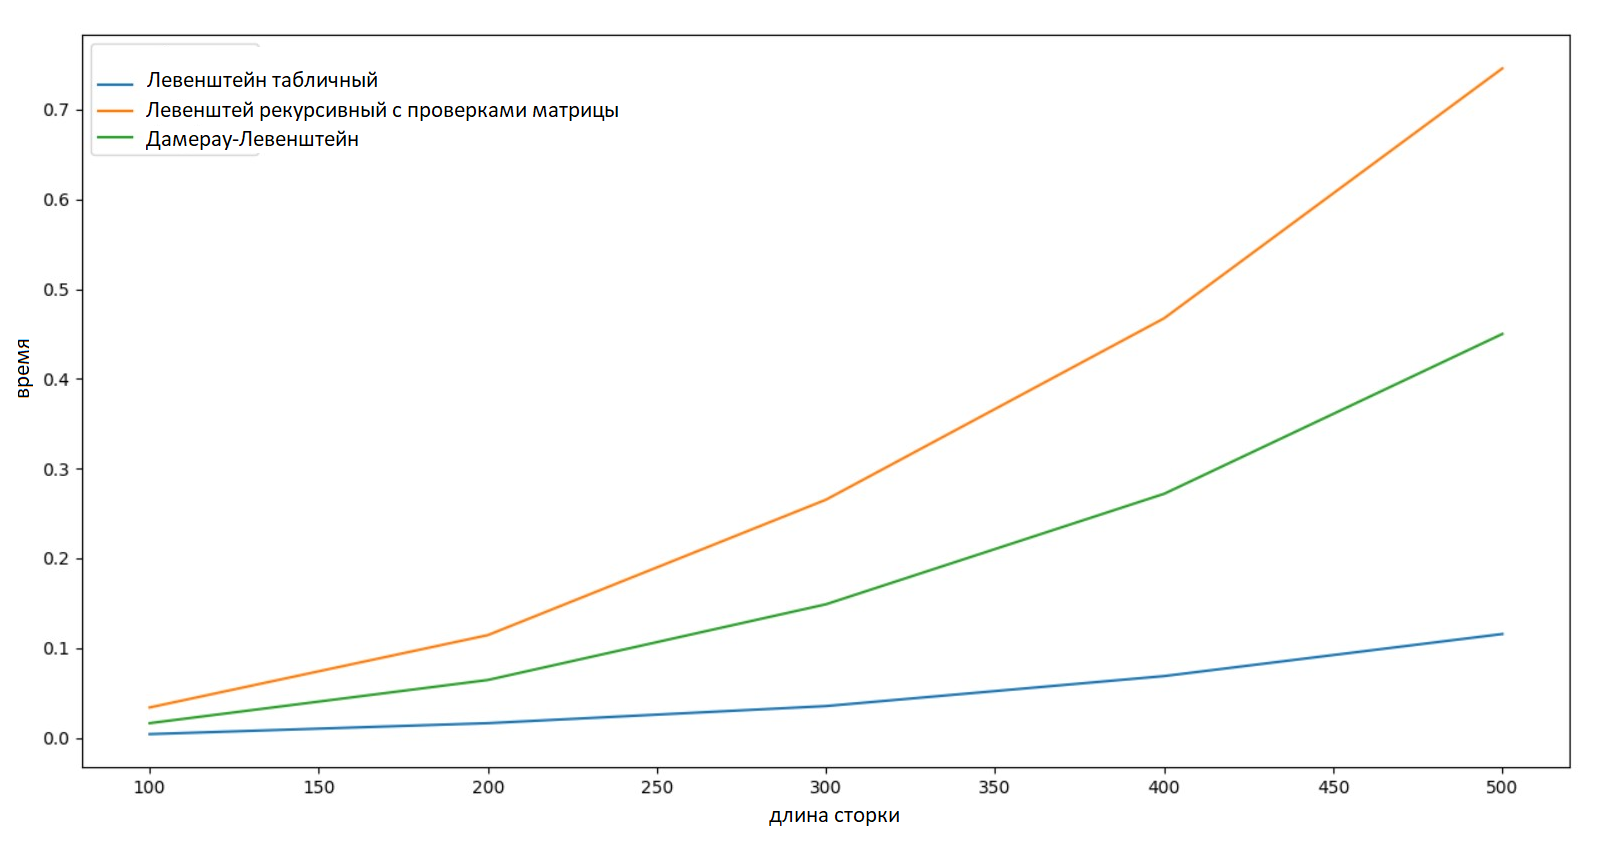
\includegraphics[scale=0.3]{time_scale_1}}
	\caption{Графики времени выполнения алгоритмов при различных длинах строки.}
\end{figure}


\section{Измерение временных характеристик для рекурсивного алгоритма Левенштейна}

Для измерения времени данных алгоритмов будет использовать рандомно генерирующиеся строки длиной от 1 до 9 с шагом 1. Для более точных измерений, для каждой длины замеры будут проводиться 50 раз и в результат будет заноситься средняя величина.
\newpage
\begin{table}[h!]
  \begin{center}
 \captionsetup{justification=raggedright}
    \caption{Результаты временных тестов.}
    \label{tab:table4}
    \begin{tabular}{c|c}
	\textbf{Длина строки} & \textbf{рекурсивного алгоритма Левенштейна}\\
      \hline
	1 & 0\\
	2 & 0\\
	3 & 0\\
	4 & 0.0003125\\
	5 & 0.0009375\\
	6 & 0.005625\\
	7 & 0.0303125\\
	8 & 0.16625\\
	9 & 0.89375\\
    \end{tabular}
  \end{center}
\end{table}

\begin{figure}[ph!]
	\center{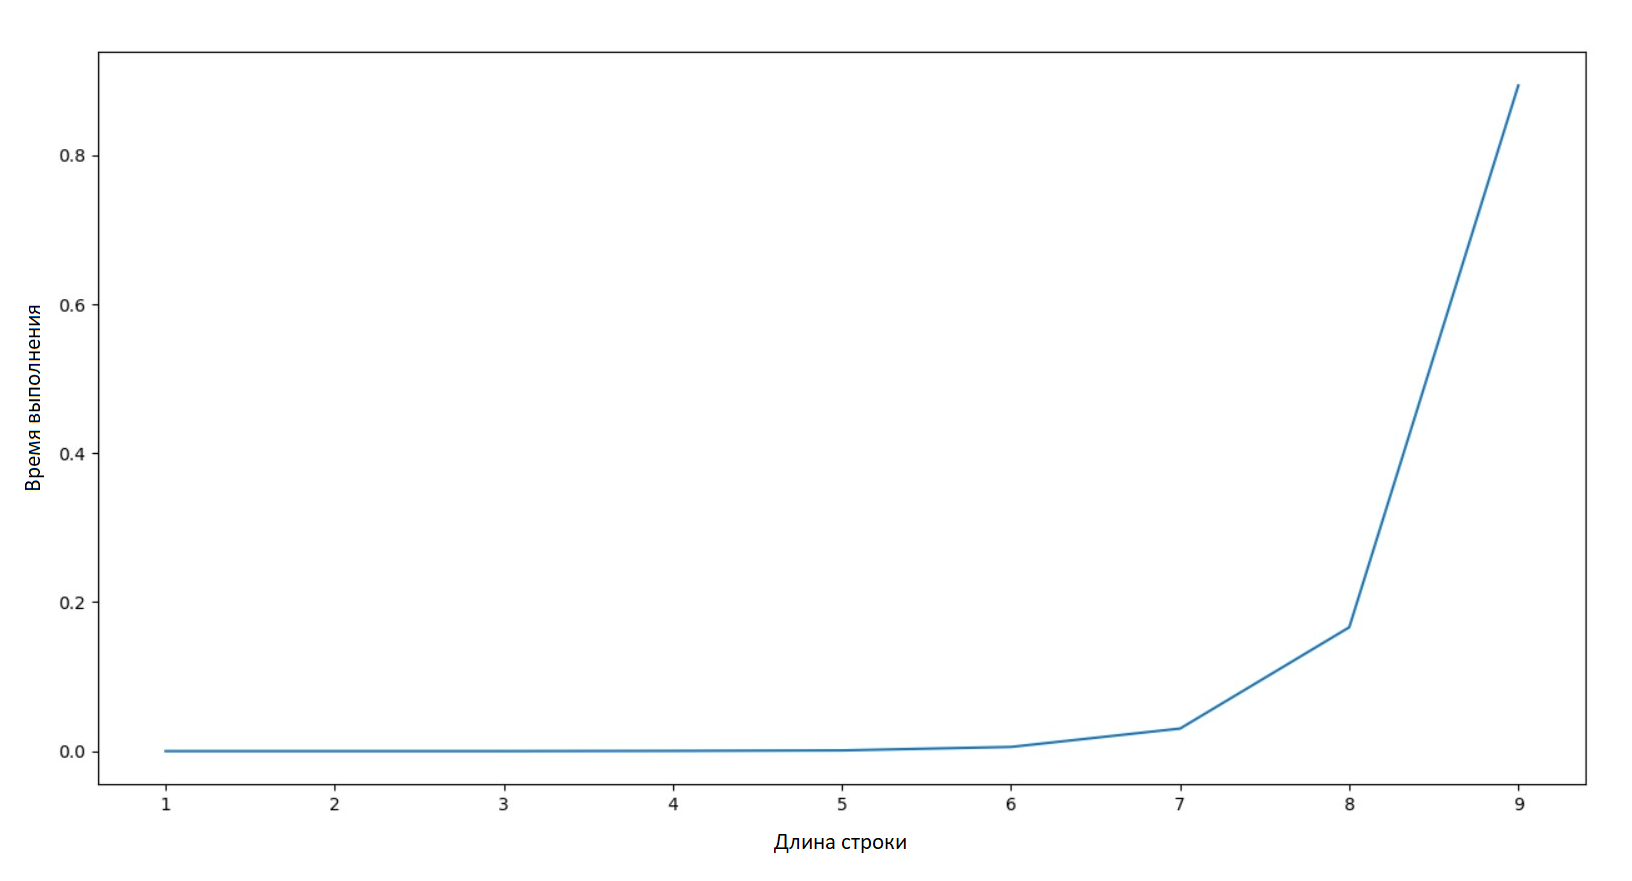
\includegraphics[scale=0.3]{time_scale_2}}
	\caption{График времени выполнения рекурсивного алгоритма Левенштейна.}
\end{figure}

\section{Вывод}
В результате эксперимента было получено, что на рандомно генерирующейся строке длиной от 1 до 9 с шагом 1, наименее времяёмким из всех рассмотренных алгоритмов является табличный алгоритм Левенштейна. В результате можно сделать вывод, что для строк длинной от 1 до 9 символов данных предпочтительно использовать табличный алгоритм Левенштейна.